
%
% Also note that the "draftcls" or "draftclsnofoot", not "draft", option
% should be used if it is desired that the figures are to be displayed in
% draft mode.
%
\documentclass[conference]{IEEEtran}
% Add the compsoc option for Computer Society conferences.
%
% If IEEEtran.cls has not been installed into the LaTeX system files,
% manually specify the path to it like:
% \documentclass[conference]{../sty/IEEEtran}



% *** CITATION PACKAGES ***
%
\usepackage{cite}

\usepackage[hmargin=1in,vmargin=1in]{geometry}


% *** GRAPHICS RELATED PACKAGES ***
%
\ifCLASSINFOpdf
  \usepackage[pdftex]{graphicx}
  % declare the path(s) where your graphic files are
  % \graphicspath{{../pdf/}{../jpeg/}}
  % and their extensions so you won't have to specify these with
  % every instance of \includegraphics
  \DeclareGraphicsExtensions{.pdf,.jpeg,.png}
\else
  % or other class option (dvipsone, dvipdf, if not using dvips). graphicx
  % will default to the driver specified in the system graphics.cfg if no
  % driver is specified.
   \usepackage[dvips]{graphicx}
  % declare the path(s) where your graphic files are
  % \graphicspath{{../eps/}}
  % and their extensions so you won't have to specify these with
  % every instance of \includegraphics
   \DeclareGraphicsExtensions{.eps}
\fi




% *** MATH PACKAGES ***
%
\usepackage[cmex10]{amsmath}



% *** SPECIALIZED LIST PACKAGES ***
%
%\usepackage{algorithmic}
% algorithmic.sty was written by Peter Williams and Rogerio Brito.
% This package provides an algorithmic environment fo describing algorithms.
% You can use the algorithmic environment in-text or within a figure
% environment to provide for a floating algorithm. Do NOT use the algorithm
% floating environment provided by algorithm.sty (by the same authors) or
% algorithm2e.sty (by Christophe Fiorio) as IEEE does not use dedicated
% algorithm float types and packages that provide these will not provide
% correct IEEE style captions. The latest version and documentation of
% algorithmic.sty can be obtained at:
% http://www.ctan.org/tex-archive/macros/latex/contrib/algorithms/
% There is also a support site at:
% http://algorithms.berlios.de/index.html
% Also of interest may be the (relatively newer and more customizable)
% algorithmicx.sty package by Szasz Janos:
% http://www.ctan.org/tex-archive/macros/latex/contrib/algorithmicx/




% *** ALIGNMENT PACKAGES ***
%
%\usepackage{array}
% Frank Mittelbach's and David Carlisle's array.sty patches and improves
% the standard LaTeX2e array and tabular environments to provide better
% appearance and additional user controls. As the default LaTeX2e table
% generation code is lacking to the point of almost being broken with
% respect to the quality of the end results, all users are strongly
% advised to use an enhanced (at the very least that provided by array.sty)
% set of table tools. array.sty is already installed on most systems. The
% latest version and documentation can be obtained at:
% http://www.ctan.org/tex-archive/macros/latex/required/tools/


%\usepackage{mdwmath}
%\usepackage{mdwtab}
% Also highly recommended is Mark Wooding's extremely powerful MDW tools,
% especially mdwmath.sty and mdwtab.sty which are used to format equations
% and tables, respectively. The MDWtools set is already installed on most
% LaTeX systems. The lastest version and documentation is available at:
% http://www.ctan.org/tex-archive/macros/latex/contrib/mdwtools/


% IEEEtran contains the IEEEeqnarray family of commands that can be used to
% generate multiline equations as well as matrices, tables, etc., of high
% quality.


%\usepackage{eqparbox}
% Also of notable interest is Scott Pakin's eqparbox package for creating
% (automatically sized) equal width boxes - aka "natural width parboxes".
% Available at:
% http://www.ctan.org/tex-archive/macros/latex/contrib/eqparbox/





% *** SUBFIGURE PACKAGES ***
%\usepackage[tight,footnotesize]{subfigure}
% subfigure.sty was written by Steven Douglas Cochran. This package makes it
% easy to put subfigures in your figures. e.g., "Figure 1a and 1b". For IEEE
% work, it is a good idea to load it with the tight package option to reduce
% the amount of white space around the subfigures. subfigure.sty is already
% installed on most LaTeX systems. The latest version and documentation can
% be obtained at:
% http://www.ctan.org/tex-archive/obsolete/macros/latex/contrib/subfigure/
% subfigure.sty has been superceeded by subfig.sty.



%\usepackage[caption=false]{caption}
%\usepackage[font=footnotesize]{subfig}
% subfig.sty, also written by Steven Douglas Cochran, is the modern
% replacement for subfigure.sty. However, subfig.sty requires and
% automatically loads Axel Sommerfeldt's caption.sty which will override
% IEEEtran.cls handling of captions and this will result in nonIEEE style
% figure/table captions. To prevent this problem, be sure and preload
% caption.sty with its "caption=false" package option. This is will preserve
% IEEEtran.cls handing of captions. Version 1.3 (2005/06/28) and later 
% (recommended due to many improvements over 1.2) of subfig.sty supports
% the caption=false option directly:
%\usepackage[caption=false,font=footnotesize]{subfig}
%
% The latest version and documentation can be obtained at:
% http://www.ctan.org/tex-archive/macros/latex/contrib/subfig/
% The latest version and documentation of caption.sty can be obtained at:
% http://www.ctan.org/tex-archive/macros/latex/contrib/caption/




% *** FLOAT PACKAGES ***
%
\usepackage{fixltx2e}
% fixltx2e, the successor to the earlier fix2col.sty, was written by
% Frank Mittelbach and David Carlisle. This package corrects a few problems
% in the LaTeX2e kernel, the most notable of which is that in current
% LaTeX2e releases, the ordering of single and double column floats is not
% guaranteed to be preserved. Thus, an unpatched LaTeX2e can allow a
% single column figure to be placed prior to an earlier double column
% figure. The latest version and documentation can be found at:
% http://www.ctan.org/tex-archive/macros/latex/base/



%\usepackage{stfloats}
% stfloats.sty was written by Sigitas Tolusis. This package gives LaTeX2e
% the ability to do double column floats at the bottom of the page as well
% as the top. (e.g., "\begin{figure*}[!b]" is not normally possible in
% LaTeX2e). It also provides a command:
%\fnbelowfloat
% to enable the placement of footnotes below bottom floats (the standard
% LaTeX2e kernel puts them above bottom floats). This is an invasive package
% which rewrites many portions of the LaTeX2e float routines. It may not work
% with other packages that modify the LaTeX2e float routines. The latest
% version and documentation can be obtained at:
% http://www.ctan.org/tex-archive/macros/latex/contrib/sttools/
% Documentation is contained in the stfloats.sty comments as well as in the
% presfull.pdf file. Do not use the stfloats baselinefloat ability as IEEE
% does not allow \baselineskip to stretch. Authors submitting work to the
% IEEE should note that IEEE rarely uses double column equations and
% that authors should try to avoid such use. Do not be tempted to use the
% cuted.sty or midfloat.sty packages (also by Sigitas Tolusis) as IEEE does
% not format its papers in such ways.






% *** Do not adjust lengths that control margins, column widths, etc. ***
% *** Do not use packages that alter fonts (such as pslatex).         ***
% There should be no need to do such things with IEEEtran.cls V1.6 and later.
% (Unless specifically asked to do so by the journal or conference you plan
% to submit to, of course. )


% correct bad hyphenation here
\hyphenation{op-tical net-works semi-conduc-tor}


\begin{document}
%
% paper title
% can use linebreaks \\ within to get better formatting as desired
\title{Ultrafast nonlinear dynamics in silicon nanocrystal-based horizontal slot waveguides}



\author{\IEEEauthorblockN{J.~Matres$^{1,*}$, A.~Mart\'inez$^1$, J.~Mart\'i$^1$,  C.~J.~Oton$^1$, J.~P.~Colonna$^2$, C.~Ratin$^2$, and J.~M.~Fedeli$^2$ }
\IEEEauthorblockA{
$^{1}$ Nanophotonics Technology Center, Universidad Polit\'ecnica de Valencia, 46022, Valencia, Spain\\
$^2$ CEA-LETI, Minatec, 17 rue des Martyrs, Grenoble, France\\
$^*$ joamatab@ntc.upv.es}
}


% make the title area
\maketitle


\begin{abstract}  %35word
%\boldmath

We present the characterization of the nonlinear-dynamics of a CMOS-compatible horizontal-slot waveguide with silicon-nanocrystals, where the temporal behavior of the phase and amplitude of the nonlinear response are simultaneously monitored. These results are complemented with four-wave-mixing measurements.

%We present the nonlinear characterization  of a CMOS-compatible slot waveguide. A phase sensitive pump and probe technique was implemented to monitor the phase and amplitude response with 1 picosecond resolution. Moreover we complement the nonlinear characterization with FWM measurements.

\end{abstract}





% For peer review papers, you can put extra information on the cover
% page as needed:
% \ifCLASSOPTIONpeerreview
% \begin{center} \bfseries EDICS Category: 3-BBND \end{center}
% \fi
%
% For peerreview papers, this IEEEtran command inserts a page break and
% creates the second title. It will be ignored for other modes.
\IEEEpeerreviewmaketitle



\section{Introduction}
Silicon photonics is a technology that is becoming competitive with alternative technologies in photonics, being its high integrability and low cost the most appealing features. Nonlinear silicon photonics is a very active research line, as devices with all-optical functionality could boost their speed with respect to their electrically-controlled counterpart. Many different nonlinear devices have been reported in the last years, such as all-optical modulators,~\cite{1} wavelength converters,~\cite{2} etc. When carrier effects are involved in these devices, the speed is limited by the carrier recombination time, which is usually in the order of 1ns. Although carrier sweeping can improve the speed,~\cite{3} nonlinear devices based on bound-electron Kerr effect are preferred, as their bandwidth does not have this limitation. Slot waveguides have demonstrated to increase the Kerr effect because of the field enhancement produced in the low-index section. Different materials have been used to fill the slot, such as organic polymers, which have allowed to demonstrate all-optical 160Gb/s demultiplexing,~\cite{4} but these materials involve non-CMOS processes and impose temperature limitations. Silicon-nanocrystal-based waveguides are fully CMOS-compatible and have a very high nonlinear coefficient,~\cite{5} and ultrafast all-optical modulation and logic gates have been recently demonstrated \cite{6}-\cite{7}. In this paper we study the nonlinear dynamics of this kind of waveguides with a time-resolved technique and we also report four-wave-mixing measurements that provide a complete nonlinear characterization.


\section{Fabrication}
Samples are fabricated starting from silicon‑-on‑-insulator (SOI) wafers with 220nm Si thickness. On top the Si layer, a 100nm--thick layer of silicon--rich silica ($ SiO_x $) was grown by PECVD, and annealed at 1200$^o$C for 1h. In this sample, the amount of silicon excess was too low to measure it with precision (probably less than 1\%). On top of that layer, a 220nm-thick layer of amorphous Si was grown by PECVD to form the top half of the waveguide. Waveguides were patterned with deep-UV lithography and etched down to the buried oxide to form channels as the ones reported in \cite{6}. Inverted tapers were added at the input and output ports to facilitate the coupling (as shown in Ref. \cite{Bakir}). The whole layout was covered with silica after the etching process.  


\section{Characterization}
The waveguides characterized in this paper are 15mm long, where the transverse-magnetic (TM) polarization mode was excited in order to magnify the electric field in the slot. Samples were characterized with a time-resolved phase-sensitive technique similar to the one described in \cite{Vallaitis2008}. In this technique, a 1ps laser pulse is divided into three pulses, one of them intense (pump) and two identical weak ones (a reference and a probe). All three pulses are combined by setting the pump very close in time to the probe, making this delay variable with a delay line. The amplitude and phase of the probe with respect to the reference pulse is measured with a heterodyne technique and monitored as a function of the delay of the pump by using a lock--in amplifier.
The nonlinear behavior was also measured with a four wave mixing technique, in which two cw beams, a pump and a signal, were amplified, combined, and coupled to the input of the waveguide. An idler signal symmetric to the signal frequency was clearly observed with an optical spectrum analyzer, as shown in Fig. \ref{fig:fwmMaxEfficiency}, and the conversion efficiency was measured as a function of the wavelength separation between pump and signal (Fig. \ref{fig:fwmBw}).


\section{Results}
\subsection{Time-resolved measurement}
In Fig. \ref{fig:p01} one can observe both Kerr and carriers effect. They produce opposite phase shifts because Kerr produces an increase in refractive index ($ \Delta n > 0 $) and carriers decrease it ($ \Delta n < 0 $).  The dynamics of each of these processes is also very different. During the pump pulse, we can see an instantaneous phase change due to Kerr effect, together with an amplitude decrease. This decrease is due to cross-absorption modulation (XAM), which consists of a two-photon absorption (TPA) process where one of the photons comes from the pump and the other comes from the probe. Once the pump pulse is gone, there is a phase response with opposite sign that remains for all the measurement range. This is due to the carrier plasma effect, also known as free-carrier dispersion (FCD). The decay time of the carriers has been measured with a direct technique and gave a result of 8~ns. This slow carrier response is expected to come from the bottom half of the waveguide, where the silicon is crystalline, as amorphous silicon has faster decay rates.
It is worth noting that a phase shift higher than $\pi/2$ is achieved with the highest pump pulse. However, there is also a power penalty due to XAM. In order to quantify the balance between XAM and Kerr effect, one can calculate the figure of merit (FOM) by using the analysis in Ref. \cite{Vallaitis}, for which no estimations of effective area or even peak power are needed. Using the same procedure, we obtained a FOM value of 0.4. In order to compare this result, we also measured a pure silicon sample of dimensions 220x500~nm, and the FOM was 0.1, which is a factor of 4 lower.


\begin{figure}[htb]
    \centering
    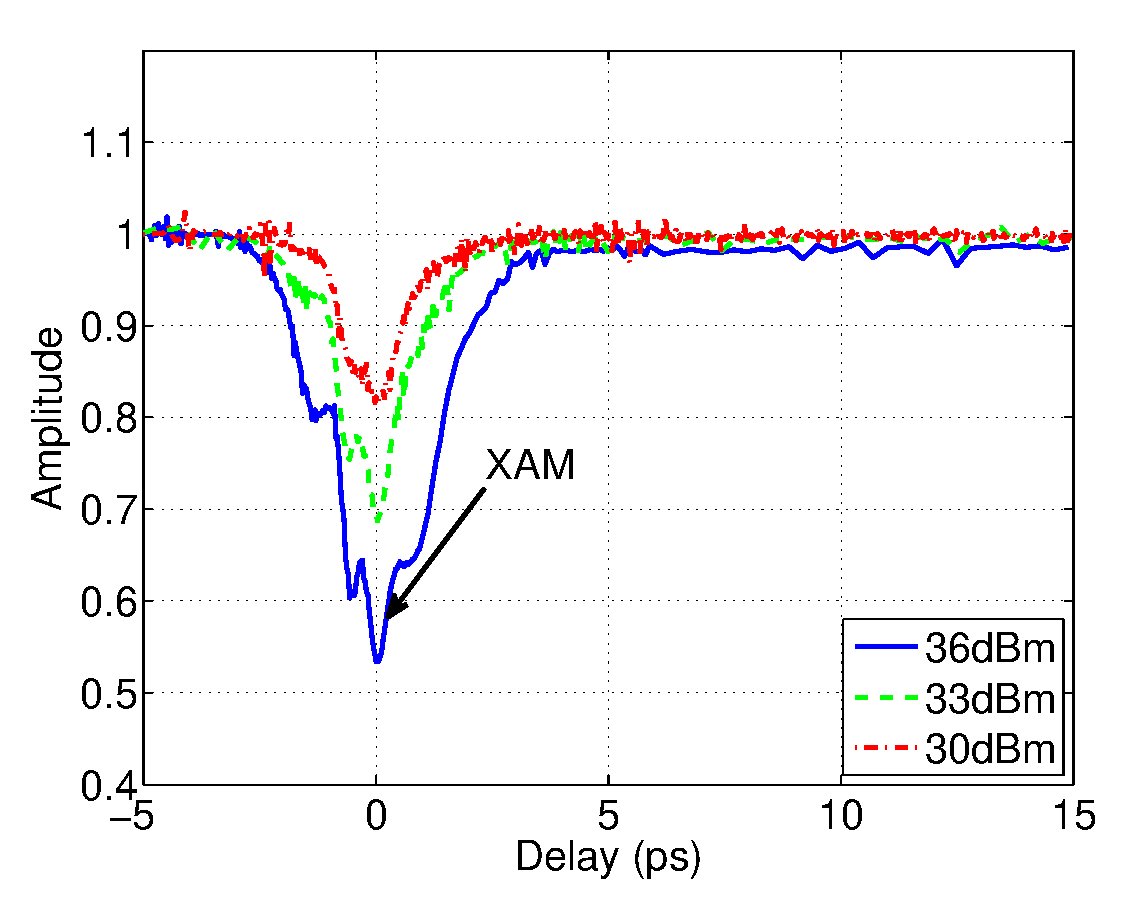
\includegraphics[width=0.45\textwidth]{p01amp_text}
	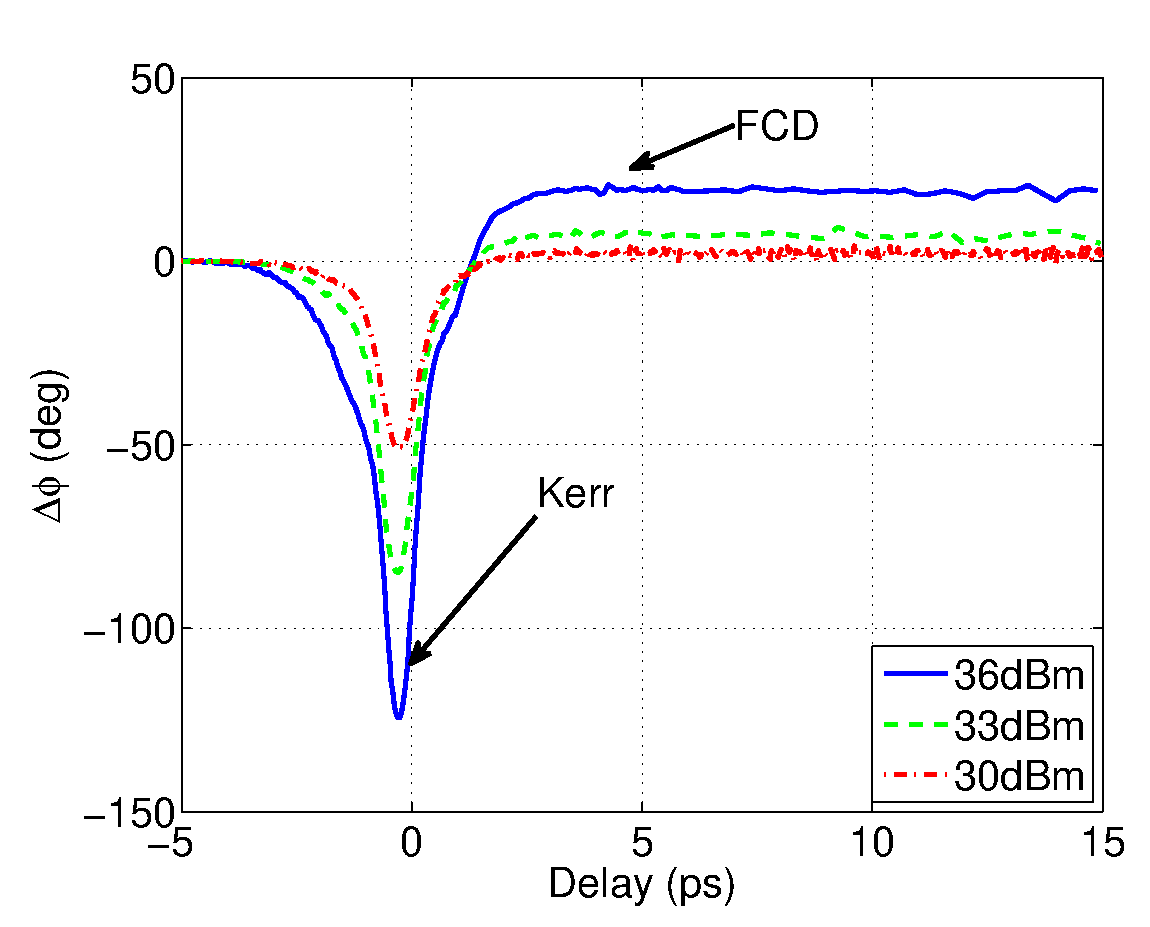
\includegraphics[width=0.47\textwidth]{p01phase_text}
    \caption{Sample response for different pump peak powers in the waveguide. Top: phase shift produced in probe pulse versus pump delay time (FCD: Free-carrier dispersion). Bottom: amplitude variation in the probe (XAM: cross absorption modulation)}
    \label{fig:p01}
\end{figure}

\begin{figure}[htb]
    \centering
    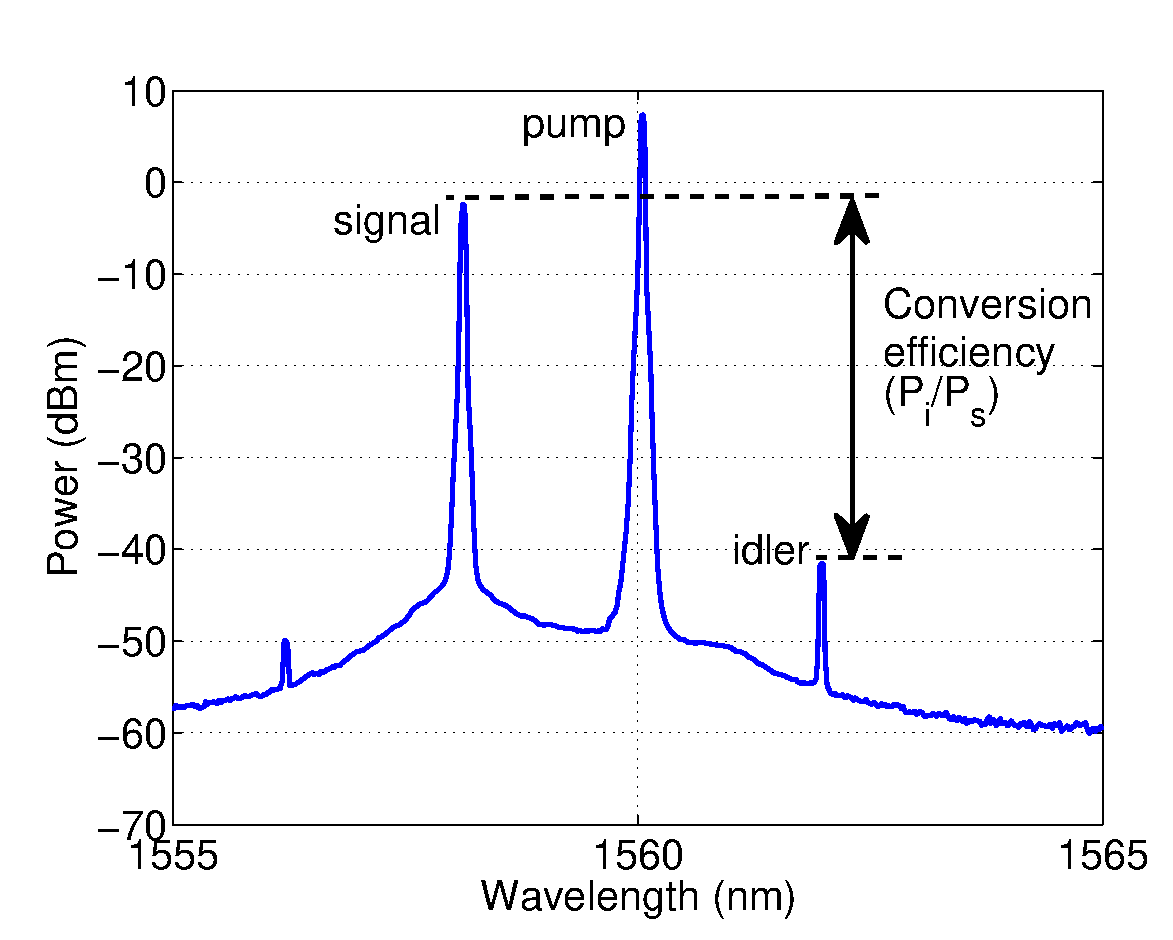
\includegraphics[width=0.45\textwidth]{maxEfficiency}
    \caption{Different signals in the FWM experiment. With pump power of 17dBm in waveguide a conversion efficiency of -39dB was measured.}
    \label{fig:fwmMaxEfficiency}
\end{figure}


\begin{figure}[htb]
    \centering
    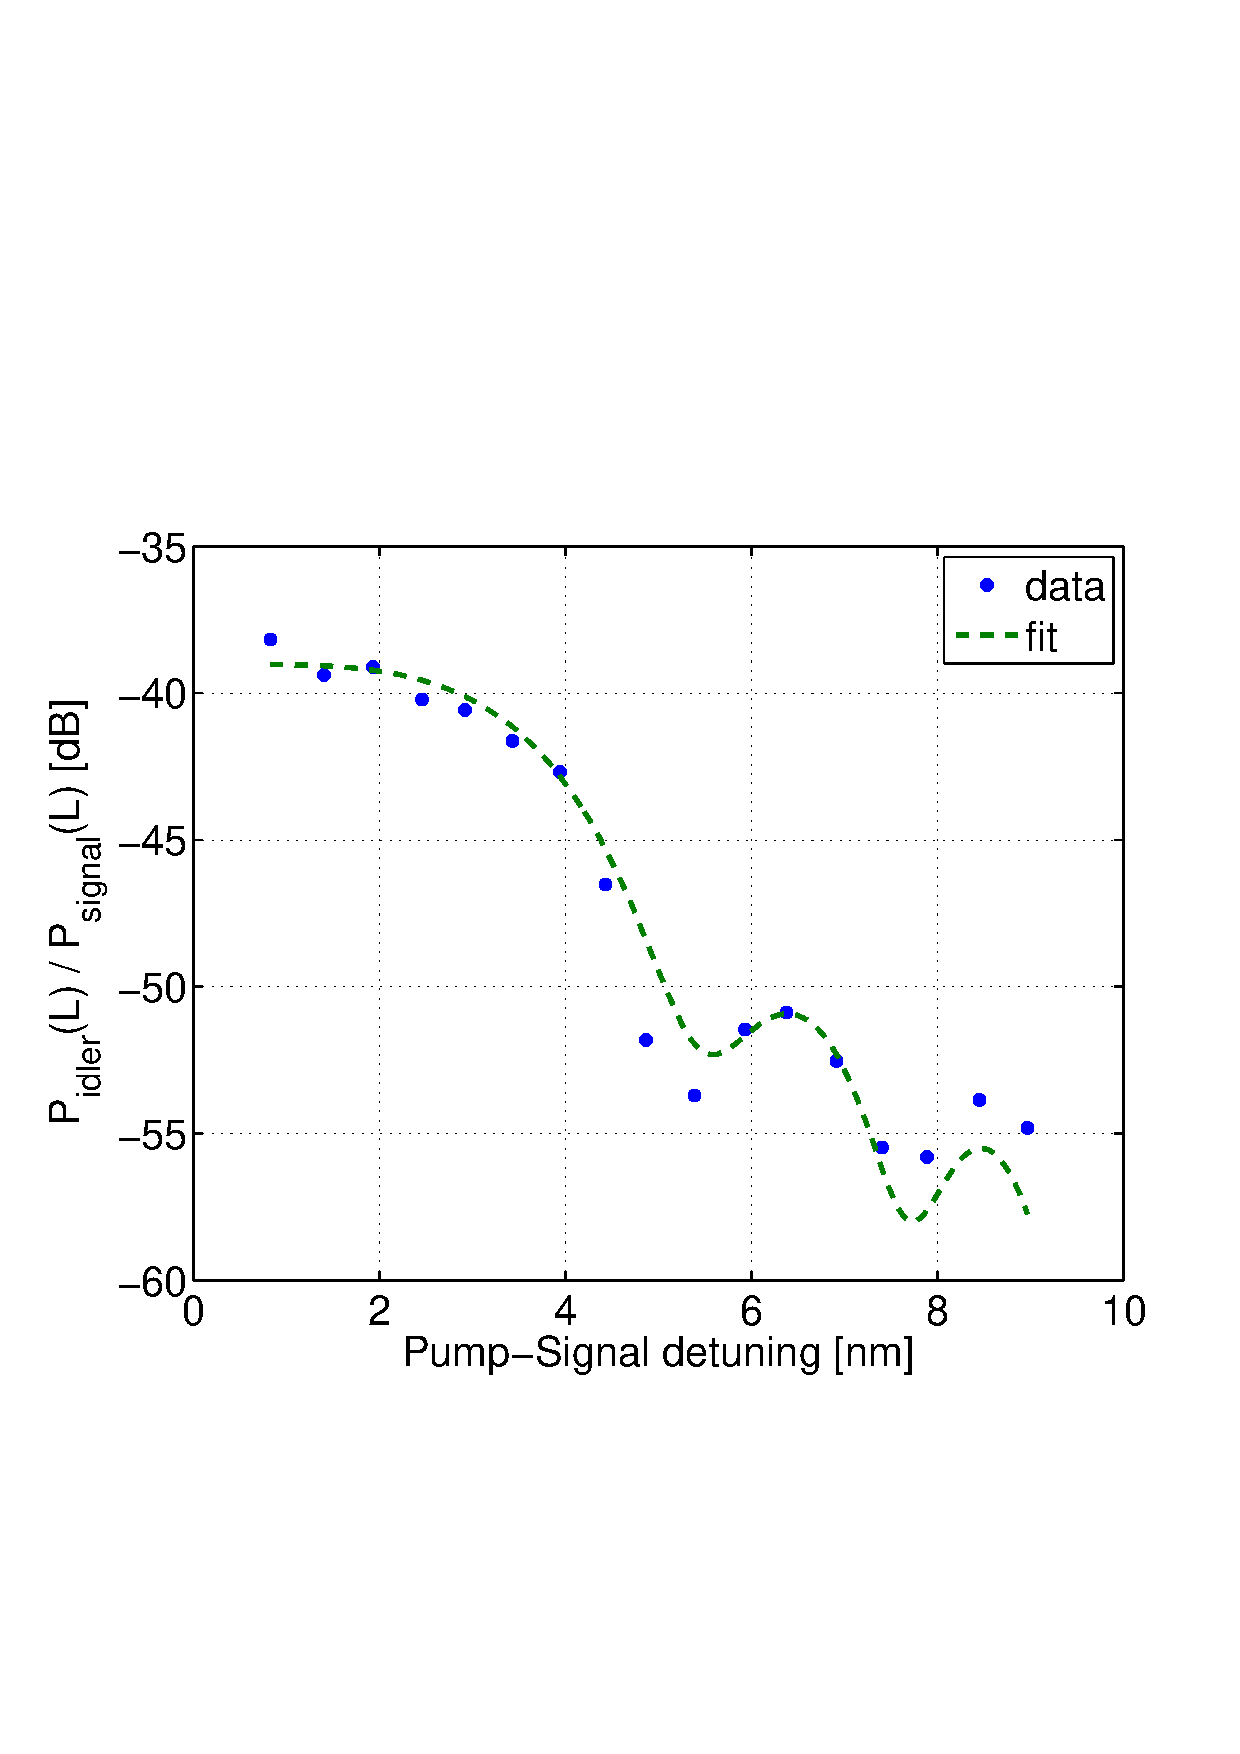
\includegraphics[width=0.45\textwidth]{fwmBwfit_big}
    \caption{$ \frac{P_{Idler}(L)}{P_{Signal}(L)}$ gives an idea of FWM Conversion efficiency when wavelength difference between signal and pump increases. Fitting to the FWM efficiency formula in paper \cite{Vallaitis} we obtain 18300ps/(nm km) dispersion and 4.1dB/cm losses.}
    \label{fig:fwmBw}
\end{figure}

\subsection{Four-wave mixing measurement}
In figure \ref{fig:fwmBw} we represent the  the $P_{idler}(L)/P_{signal}(L)$ ratio, that gives an idea of the conversion efficiency of the idler generated changing the wavelength difference between pump $ (\lambda_p) $ and signal $ (\lambda_s) $. Assuming that at these power levels TPA is negligible, one can fit the results to the equation shown in Ref.~\cite{Vallaitis} for the FWM efficiency $ \eta $ formula:


\begin{equation}
	\eta ^2=\frac{\alpha_0^2}{\alpha_0^2+\Delta \beta^2}\left[ 1+ 4e^{-\alpha_0L}\frac{sin^2(L\Delta\beta/2)}{(1-e^{-\alpha_0L})^2} \right] \nonumber	
\end{equation}

where $ \Delta\beta $ for a detuning $ \Delta\lambda = \lambda_p-\lambda_s$ is given by:

\begin{equation}
	\Delta \beta=\frac{2\pi cD_2}{\lambda_p^2}\Delta\lambda^2 \nonumber
\end{equation}

%and $ D_2 $ is the group velocity dispersion.

The equation agrees with the experimental curve, obtaining a chromatic dispersion $ (D_2) $ of 18300ps/(nm km) and a value of propagation loss $ (\alpha_0) $ of 4.1~dB/cm. The sign of the dispersion has been extracted from independent dispersion measurements performed with an interferometric setup. The value obtained by this other  method is -18700~ps/(nm~km), which agrees with the aforementioned result, and shows that the dispersion is negative (normal dispersion). This relatively high dispersion value is the cause of having a bandwidth of only about 5.5~nm. This is because the geometry of the waveguide was not optimized to minimize dispersion at 1.55~$\mu$m. Dispersion engineering may prove useful to increase the conversion bandwidth of this waveguide, as studied in Ref. \cite{Caraquitena}.

%Furthermore, one can also calculate the real part of the $\gamma$ coefficient in the waveguide given the conversion efficiency when detuning tends to zero. By using the equation $ \frac{P_i(L)}{P_s(L)}=(\eta Re\{\gamma\}P_P(0)L_{eff})^2  $, we obtain $\gamma=27~W^{-1}m^{-1}$.

Furthermore, one can also calculate the real part of the $\gamma$ coefficient in the waveguide given the conversion efficiency when detuning tends to zero. By using the equation:

\begin{equation}
	\frac{P_i(L)}{P_s(L)}=(\eta Re\{\gamma\}P_P(0)L_{eff})^2  \nonumber	
\end{equation}

where $ L_{eff} $ is the effective waveguide length, $ P_i(L) $, $ P_s(L) $ are the idler and output signal powers respectively, and $ P_P(0) $ is the input pump power,

\begin{equation}
	L_{eff}=\frac{1-e^{-\alpha_0L}}{\alpha_0}  \nonumber	
\end{equation}


we obtain $\gamma=27~W^{-1}m^{-1}$.


\section{Conclusion}
We have shown the characterization of the ultrafast dynamics of the nonlinear response of a silicon nanocrystal-based horizontal slot waveguide. A time-resolved pump and probe technique allowed to clearly distinguish the Kerr effect and XAM mechanisms, which are instantaneous, from the carrier effect, which takes place after the pulse has left the waveguide and lasts for several nanoseconds. On the other hand, four-wave-mixing measurements show wavelength conversion with a bandwidth of 5.5nm, due to the high normal dispersion of the waveguide, which was -18300~ps/(nm~km). A higher conversion bandwidth would therefore require dispersion engineering. 

% conference papers do not normally have an appendix

% use section* for acknowledgement
\section*{Acknowledgments}
%This work has been sponsored by the Spanish Science and Innovation Ministry through SINADEC (TEC2008-06333) and DEMOTEC (TEC2008-06360) contracts and by Generalitat Valenciana through PROMETEO-2010-087 RD Excellence Program (NANOMET).

We acknowledge financial support from the EU project PHOLOGIC (FP6-IST-NMP-017158), the Spanish Ministry of Science and Innovation through contracts SINADEC (TEC2008- 06333) and DEMOTEC (TEC2008-06360) and from Generalitat Valenciana through PROMETEO-2010-087 RD Excellence Program (NANOMET).



%\begin{figure}[!t]
 %   \centering
  %  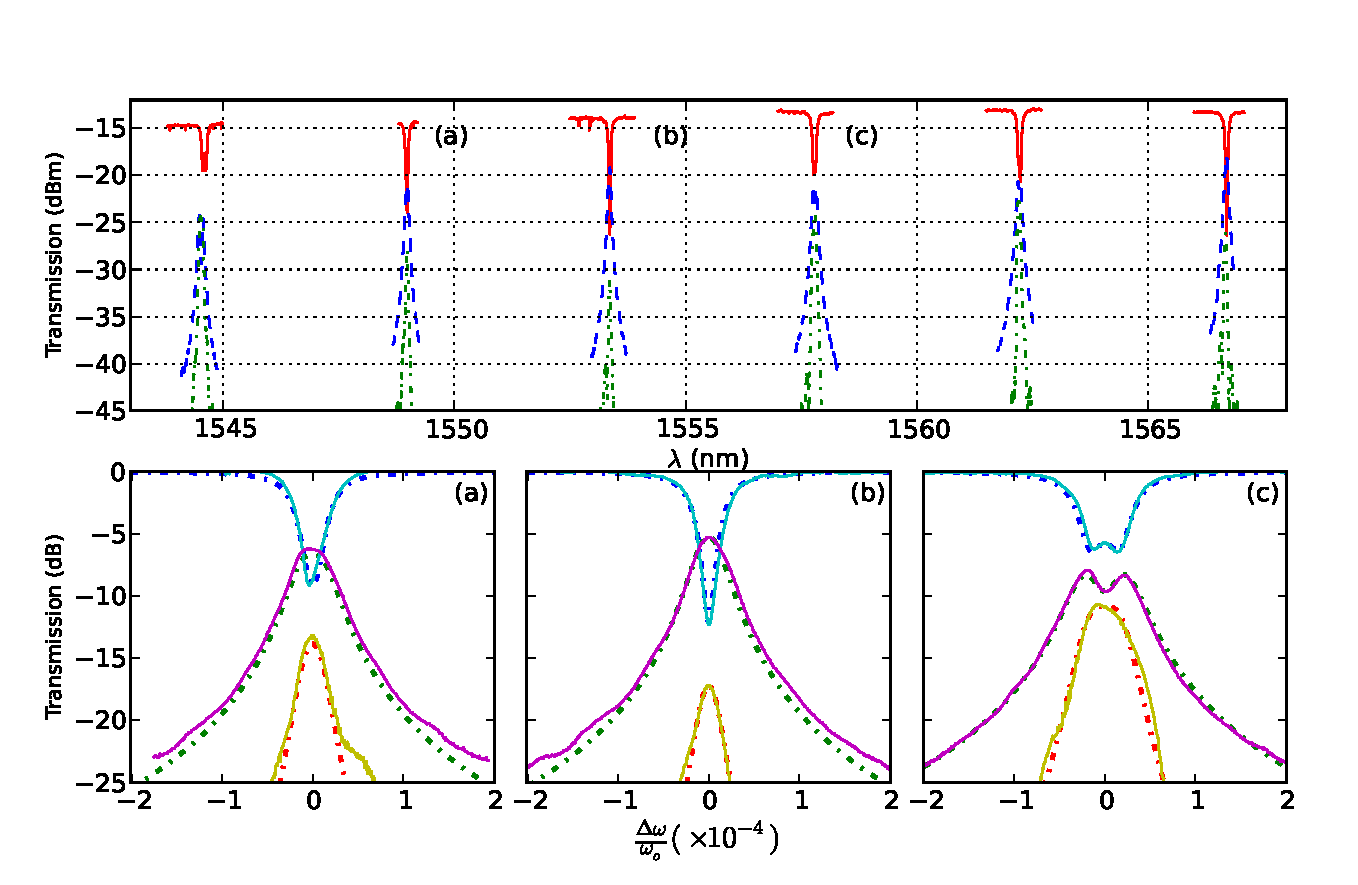
\includegraphics[width=1.\textwidth]{espectro_2.eps}
   % \caption{Solid curves are measurements of the throught port, while the dashed and dot-dashed lines are the drop and counter-drop ports respectively}
    %\label{fig:espectro}
%\end{figure}

% Note that \label must occur AFTER (or within) \caption.
% For figures, \caption should occur after the \includegraphics.
% Note that IEEEtran v1.7 and later has special internal code that
% is designed to preserve the operation of \label within \caption
% even when the captionsoff option is in effect. However, because
% of issues like this, it may be the safest practice to put all your
% \label just after \caption rather than within \caption{}.
%
% Reminder: the "draftcls" or "draftclsnofoot", not "draft", class
% option should be used if it is desired that the figures are to be
% displayed while in draft mode.
%
%\begin{figure}[!t]
%\centering
%\includegraphics[width=2.5in]{myfigure}
% where an .eps filename suffix will be assumed under latex, 
% and a .pdf suffix will be assumed for pdflatex; or what has been declared
% via \DeclareGraphicsExtensions.
%\caption{Simulation Results}
%\label{fig_sim}
%\end{figure}

% Note that IEEE typically puts floats only at the top, even when this
% results in a large percentage of a column being occupied by floats.


% An example of a double column floating figure using two subfigures.
% (The subfig.sty package must be loaded for this to work.)
% The subfigure \label commands are set within each subfloat command, the
% \label for the overall figure must come after \caption.
% \hfil must be used as a separator to get equal spacing.
% The subfigure.sty package works much the same way, except \subfigure is
% used instead of \subfloat.
%
%\begin{figure*}[!t]
%\centerline{\subfloat[Case I]\includegraphics[width=2.5in]{subfigcase1}%
%\label{fig_first_case}}
%\hfil
%\subfloat[Case II]{\includegraphics[width=2.5in]{subfigcase2}%
%\label{fig_second_case}}}
%\caption{Simulation results}
%\label{fig_sim}
%\end{figure*}
%
% Note that often IEEE papers with subfigures do not employ subfigure
% captions (using the optional argument to \subfloat), but instead will
% reference/describe all of them (a), (b), etc., within the main caption.


% An example of a floating table. Note that, for IEEE style tables, the 
% \caption command should come BEFORE the table. Table text will default to
% \footnotesize as IEEE normally uses this smaller font for tables.
% The \label must come after \caption as always.
%
%\begin{table}[!t]
%% increase table row spacing, adjust to taste
%\renewcommand{\arraystretch}{1.3}
% if using array.sty, it might be a good idea to tweak the value of
% \extrarowheight as needed to properly center the text within the cells
%\caption{An Example of a Table}
%\label{table_example}
%\centering
%% Some packages, such as MDW tools, offer better commands for making tables
%% than the plain LaTeX2e tabular which is used here.
%\begin{tabular}{|c||c|}
%\hline
%One & Two\\
%\hline
%Three & Four\\
%\hline
%\end{tabular}
%\end{table}


% Note that IEEE does not put floats in the very first column - or typically
% anywhere on the first page for that matter. Also, in-text middle ("here")
% positioning is not used. Most IEEE journals/conferences use top floats
% exclusively. Note that, LaTeX2e, unlike IEEE journals/conferences, places
% footnotes above bottom floats. This can be corrected via the \fnbelowfloat
% command of the stfloats package.




% trigger a \newpage just before the given reference
% number - used to balance the columns on the last page
% adjust value as needed - may need to be readjusted if
% the document is modified later
%\IEEEtriggeratref{8}
% The "triggered" command can be changed if desired:
%\IEEEtriggercmd{\enlargethispage{-5in}}

% references section

% can use a bibliography generated by BibTeX as a .bbl file
% BibTeX documentation can be easily obtained at:
% http://www.ctan.org/tex-archive/biblio/bibtex/contrib/doc/
% The IEEEtran BibTeX style support page is at:
% http://www.michaelshell.org/tex/ieeetran/bibtex/
%\bibliographystyle{IEEEtran}
% argument is your BibTeX string definitions and bibliography database(s)
%\bibliography{IEEEabrv,../bib/paper}
%
% <OR> manually copy in the resultant .bbl file
% set second argument of \begin to the number of references
% (used to reserve space for the reference number labels box)

\begin{thebibliography}{99}

\bibitem{1}
V.R. Almeida, C.A. Barrios, R.R. Panepucci, and M. Lipson, “All-optical control of light on a silicon chip,” Nature, vol. 431, 2004, p. 1081–1084.

\bibitem{2}
B.G. Lee, A. Biberman, A.C. Turner-Foster, M. a Foster, M. Lipson, A.L. Gaeta, and K. Bergman, “Demonstration of Broadband Wavelength Conversion at 40 Gb/s in Silicon Waveguides,” IEEE Photonics Technology Letters, vol. 21, Feb. 2009, pp. 182-184.

\bibitem{3}
A.C. Turner-Foster, M. a Foster, J.S. Levy, C.B. Poitras, R. Salem, A.L. Gaeta, and M. Lipson, “Ultrashort free-carrier lifetime in low-loss silicon nanowaveguides.,” Optics express, vol. 18, Feb. 2010, pp. 3582-3591.

\bibitem{4}
C. Koos, P. Vorreau, T. Vallaitis, P. Dumon, W. Bogaerts, R. Baets, B. Esembeson, I. Biaggio, T. Michinobu, F. Diederich, W. Freude, and J. Leuthold, “All-optical high-speed signal processing with silicon–organic hybrid slot waveguides,” Nature Photonics, vol. 3, Mar. 2009, pp. 216-219.

\bibitem{5}
R. Spano, N. Daldosso, M. Cazzanelli, L. Ferraioli, L. Tartara, J. Yu, V. Degiorgio, E. Giordana, J.M. Fedeli, and L. Pavesi, “Bound electronic and free carrier nonlinearities in Silicon nanocrystals at 1550nm.,” Optics express, vol. 17, Mar. 2009, pp. 3941-50.

\bibitem{6}
A. Mart\'inez, J. Blasco, P. Sanchis, J.V. Gal\'an, J. Garc\'ia-Rup\'erez, E. Jordana, P. Gautier, Y. Lebour, S. Hern\'andez, R. Guider, N. Daldosso, B. Garrido, J.M. Fedeli, L. Pavesi, and J. Mart\'i, “Ultrafast all-optical switching in a silicon-nanocrystal-based silicon slot waveguide at telecom wavelengths.,” Nano letters, vol. 10, Apr. 2010, pp. 1506-1511.

\bibitem{7}
C. J. Oton, J. Matres, A. Mart\'inez, P. Sanchis, J. P. Colonna, C. Ratin, J. M. Fedeli, J. Mart\'i, “Ultrafast all-optical logic gates with silicon nanocrystal-based slot waveguides”, Group IV Photonics Conference (2010).

\bibitem{Bakir}
 B.B. Bakir, R. Orobtchouk, P. Lyan, C. Porzier, and A. Roman, “Low-Loss ( $< 1 dB$) and Polarization-Insensitive Edge Fiber Couplers Fabricated on 200-mm Silicon-on-Insulator Wafers,” Technology, vol. 22, 2010, pp. 739-741.

\bibitem{Vallaitis2008}
T. Vallaitis, C. Koos, R. Bonk, W. Freude, M. Laemmlin, C. Meuer, D. Bimberg, and J. Leuthold, “Slow and fast dynamics of gain and phase in a quantum dot semiconductor optical amplifier.,” Optics express, vol. 16, Jan. 2008, pp. 170-8.

\bibitem{Vallaitis}
T. Vallaitis, S. Bogatscher, L. Alloatti, P. Dumon, R. Baets, M.L. Scimeca, I. Biaggio, F. Diederich, C. Koos, W. Freude, and J. Leuthold, “Optical properties of highly nonlinear silicon-organic hybrid (SOH) waveguide geometries.,” Optics express, vol. 17, Sep. 2009, pp. 17357-68.


\bibitem{Caraquitena}
S. Mas, J. Caraquitena, J.V. Gal\'an, P. Sanchis, and J. Mart\'i, “Tailoring the dispersion behavior of silicon nanophotonic slot waveguides.,” Optics Express, vol. 18, Sep. 2010, pp. 20839-20844.

\end{thebibliography}


%\begin{figure}[!h]gi
%    \centering
%    \includegraphics[width=1.0\textwidth]{ajuste_1553.eps}
%    \caption{Layout of the rings.}
%    \label{fig:add_drop_ring}
%\end{figure}

% that's all folks
\end{document}

%ccurring within multiline equations. Use:
%\interdisplaylinepenalty=2500
% after loading amsmath to restore such page breaks as IEEEtran.cls normally
% does. amsmath.sty is already installed on most LaTeX systems. The latest
% version and documentation can be obtained at:
% http://www.ctan.org/tex-archive/macros/latex/required/amslatex/math/


